\documentclass[11pt]{beamer}
 \usetheme{Szeged}
 \usepackage[utf8]{inputenc}
 \usepackage[magyar]{babel}
 \usepackage[T1]{fontenc}
 \usepackage{graphicx}
 \usepackage{hyperref}
 \author{Tipográfiai rendszerek - \TeX}
 \title{Felsorolások, táblázatok, képek \\ úsztatott objektumok és hivatkozások}
 \date{2021.03.03.}
 
 \newcommand{\tbs}{\textbackslash}

 \begin{document}
 
 \begin{frame}
 \titlepage
 \end{frame}
 
\begin{frame}{Hasznos oldalak}
\begin{itemize}
\item	OverLeaf súgó: \href{https://overleaf.com/learn/latex}{http://overleaf.com/learn/\LaTeX{}}
\item 	\TeX{}.StackExchange: \href{https://tex.stackexchange.com}{http://\TeX{}.stackexchange.com}
\end{itemize}
\end{frame}

 \begin{frame}{Felsorolás / lista - itemize}
 \begin{itemize}
\item Formátum: \\ 
	\tbs begin\{itemize\} \\ 
	\tbs item \textit{adat1} \\ 
	\tbs item \textit{adat2} \\ 
	\tbs item \textit{adat3} \\ 
	\tbs end\{itemize\} közt
\item Opcionális paraméter is adható: \tbs item[op. par.] \textit{adat1}
	\begin{itemize}
	\item Ekkor az a karakter / karakter sorozat jelenik meg a szöveg előtt, amit megadtunk
	\end{itemize}
\item	A listák egymásba ágyazhatóak. Ekkor egy újabb itemize környezetet kell létrehoznunk
 \end{itemize}
 \end{frame}
 
 
\begin{frame}{Felsorolás - enumerate (,,számláló'')\footnote{szabad fordítás!}}
 \begin{itemize}
\item Formátum: \\ 
	\tbs begin\{enumerate\} \\ 
	\tbs item \textit{adat1} \\ 
	\tbs item \textit{adat2} \\ 
	\tbs item \textit{adat3} \\ 
	\tbs end\{enumerate\} közt
\item Opcionális paraméter is adható: \tbs item[op. par.] \textit{adat1}
	\begin{itemize}
	\item Ekkor az a karakter / karakter sorozat jelenik meg a szöveg előtt, amit megadtunk
	\item Ilyenkor a számozás átugorja az adott elemet.
	\end{itemize}
\item	A számozott listák egymástól függetlenek.
\item	Új számozott lista az egyestől fog kezdődni.
 \end{itemize}
\end{frame}

\begin{frame}
\begin{itemize}
\item opcionális paramétert megadva, a számozás is változtatható:
\item \tbs begin{enumerate}[paraméter]
	\begin{itemize}
	\item a
	\item A
	\item i
	\item I
	\end{itemize}
\end{itemize}
\end{frame}

\begin{frame}{Egymásba ágyazhatóság}
\begin{itemize}
\item	A felsorolásokat egymásba lehet ágyazni
	\begin{itemize}
	\item Ilyenkor mindig egy új itemize / enumerate környezetet kell létrehozni
	\end{itemize}
\item	Az elemek előtt megjelenő szimbólumokat / számokat át lehet definiálni
\end{itemize}
\end{frame}

\begin{frame}{Táblázatok}
\begin{itemize}
\item	\tbs begin\{tabular\}\{oszlopok száma és tulajdonsága\} \\ 
		elem1 \& elem2 \tbs \tbs \\ 
		elem3 \& elem4  \\ 
		\tbs end\{tabular\} \\
\item	az oszlopok számát és elrendezését az l, r, c karakterekkel határozzuk meg
		\begin{itemize}
		\item	left
		\item	right
		\item	center
		\end{itemize}
\item	a cellákat az \& karakterrel választjuk el
\item	a sorokat a \tbs \tbs -el választjuk el
\item	a függőleges elválasztó vonalakat a | karakterrel adjuk meg. Pl. c|c|c
\item	a vízszintes elválasztó vonalakat a \tbs hline-el adjuk meg
\end{itemize}
\end{frame}

\begin{frame}[fragile]
\begin{center}
\begin{tabular}{|c|c|}
\hline 
elem1 & elem2 \\ 
\hline 
elem3 & elem4 \\ 
\hline 
\end{tabular} 
\end{center}
\vspace{2cm}
\begin{verbatim}
\begin{tabular}{|c|c|}
\hline 
elem1 & elem2 \\ 
\hline 
elem3 & elem4 \\ 
\hline 
\end{tabular}
\end{verbatim}
\end{frame}

\begin{frame}[fragile]
\begin{itemize}
\item	Az elválasztókból többet is egymásba lehet ágyazni.
\item	Ilyenkor csak ismételni kell az elválasztót
\item	Pl.:
		\begin{itemize}
		\item	c||c|c
		\item	\tbs hline \tbs hline
		\end{itemize}
\end{itemize}
\vspace{10px}
\begin{center}
\begin{tabular}{|c||c|}
\hline 
elem1 & elem2 \\ 
\hline \hline
elem3 & elem4 \\ 
\hline 
\end{tabular} 
\end{center}
\vspace{10px}
\begin{verbatim}
\begin{tabular}{|c||c|}
\hline 
elem1 & elem2 \\ 
\hline \hline
elem3 & elem4 \\ 
\hline 
\end{tabular}
\end{verbatim}
\end{frame}

\begin{frame}{Cellák összevonása táblázatoknál - sorban}
\begin{itemize}
\item ezt a \textbf{\tbs multicolumn\{mennyit\}\{igazítás\}\{címke\}} paranccsal tudjuk megtenni
\item a mennyit-ben az összevonandó cellák számát kell megadnunk
\item az igazításban a tartalom igazítását, valamint az elválasztókat
\item a címkénél pedig a cella tartalmát kell megadnunk
\end{itemize}
\end{frame}
\begin{frame}[fragile]{Cellák összevonása táblázatoknál - sorban}
\begin{center}
\begin{tabular}{|c|c|c|c|}
\hline 
\multicolumn{3}{|c|}{Címke} & Akármi \\ 
\hline 
Egy & Kettő & Három & Négy \\ 
\hline 
Öt & Hat & Hét & Nyolc \\ 
\hline 
\end{tabular}
\end{center}
\vspace{0.5cm}
\begin{verbatim}
\begin{tabular}{|c|c|c|c|}
\hline 
\multicolumn{3}{|c|}{Címke} & Akármi \\ 
\hline 
Egy & Kettő & Három & Négy \\ 
\hline 
Öt & Hat & Hét & Nyolc \\ 
\hline 
\end{tabular} 
\end{verbatim}
\end{frame}
 
\begin{frame}{input és include}
\begin{itemize}
\item	Ezekkel lehet a \TeX{} dokumentumainkhoz hozzáfűzni egyéb \TeX{} dokumentumokat
\item	\tbs include\{tex\_fajl\} - új oldalon kezdi a beillesztést
\item	\tbs input\{tex\_fajl\} - egyszerű beillesztés
\item	kiterjesztést nem írunk!
\end{itemize}
\end{frame}

\begin{frame}{Kép beillesztése}
\begin{itemize}
\item Ehhez kell a \textbf{graphicx} csomag is!
\item Képet a \textbf{\tbs includegraphics[scale=•]\{kep\_neve\}} paranccsal illeszthetünk be
\item A képnek az útvonalát, vagy mappán belül a nevét kell megadni, kiterjesztés nélkül
\item A scale határozza meg a kép nagyságát: \\ 1 = 100\%, 0.5 = 50\%, \dots
\item Használhatjuk a \textbf{width=\tbs textwidth} parancsot is, ekkor a szöveg szélességével lesz egyenlő a kép szélessége
\item a \textbf{0.X\tbs textwidth} pedig a szöveg szélességéhez mérten csökkenti a kép méretét.
\item használható még a \textbf{\tbs width=\dots cm} és \textbf{\tbs height=\dots cm}
\end{itemize}
\end{frame}

\begin{frame}
\begin{figure}
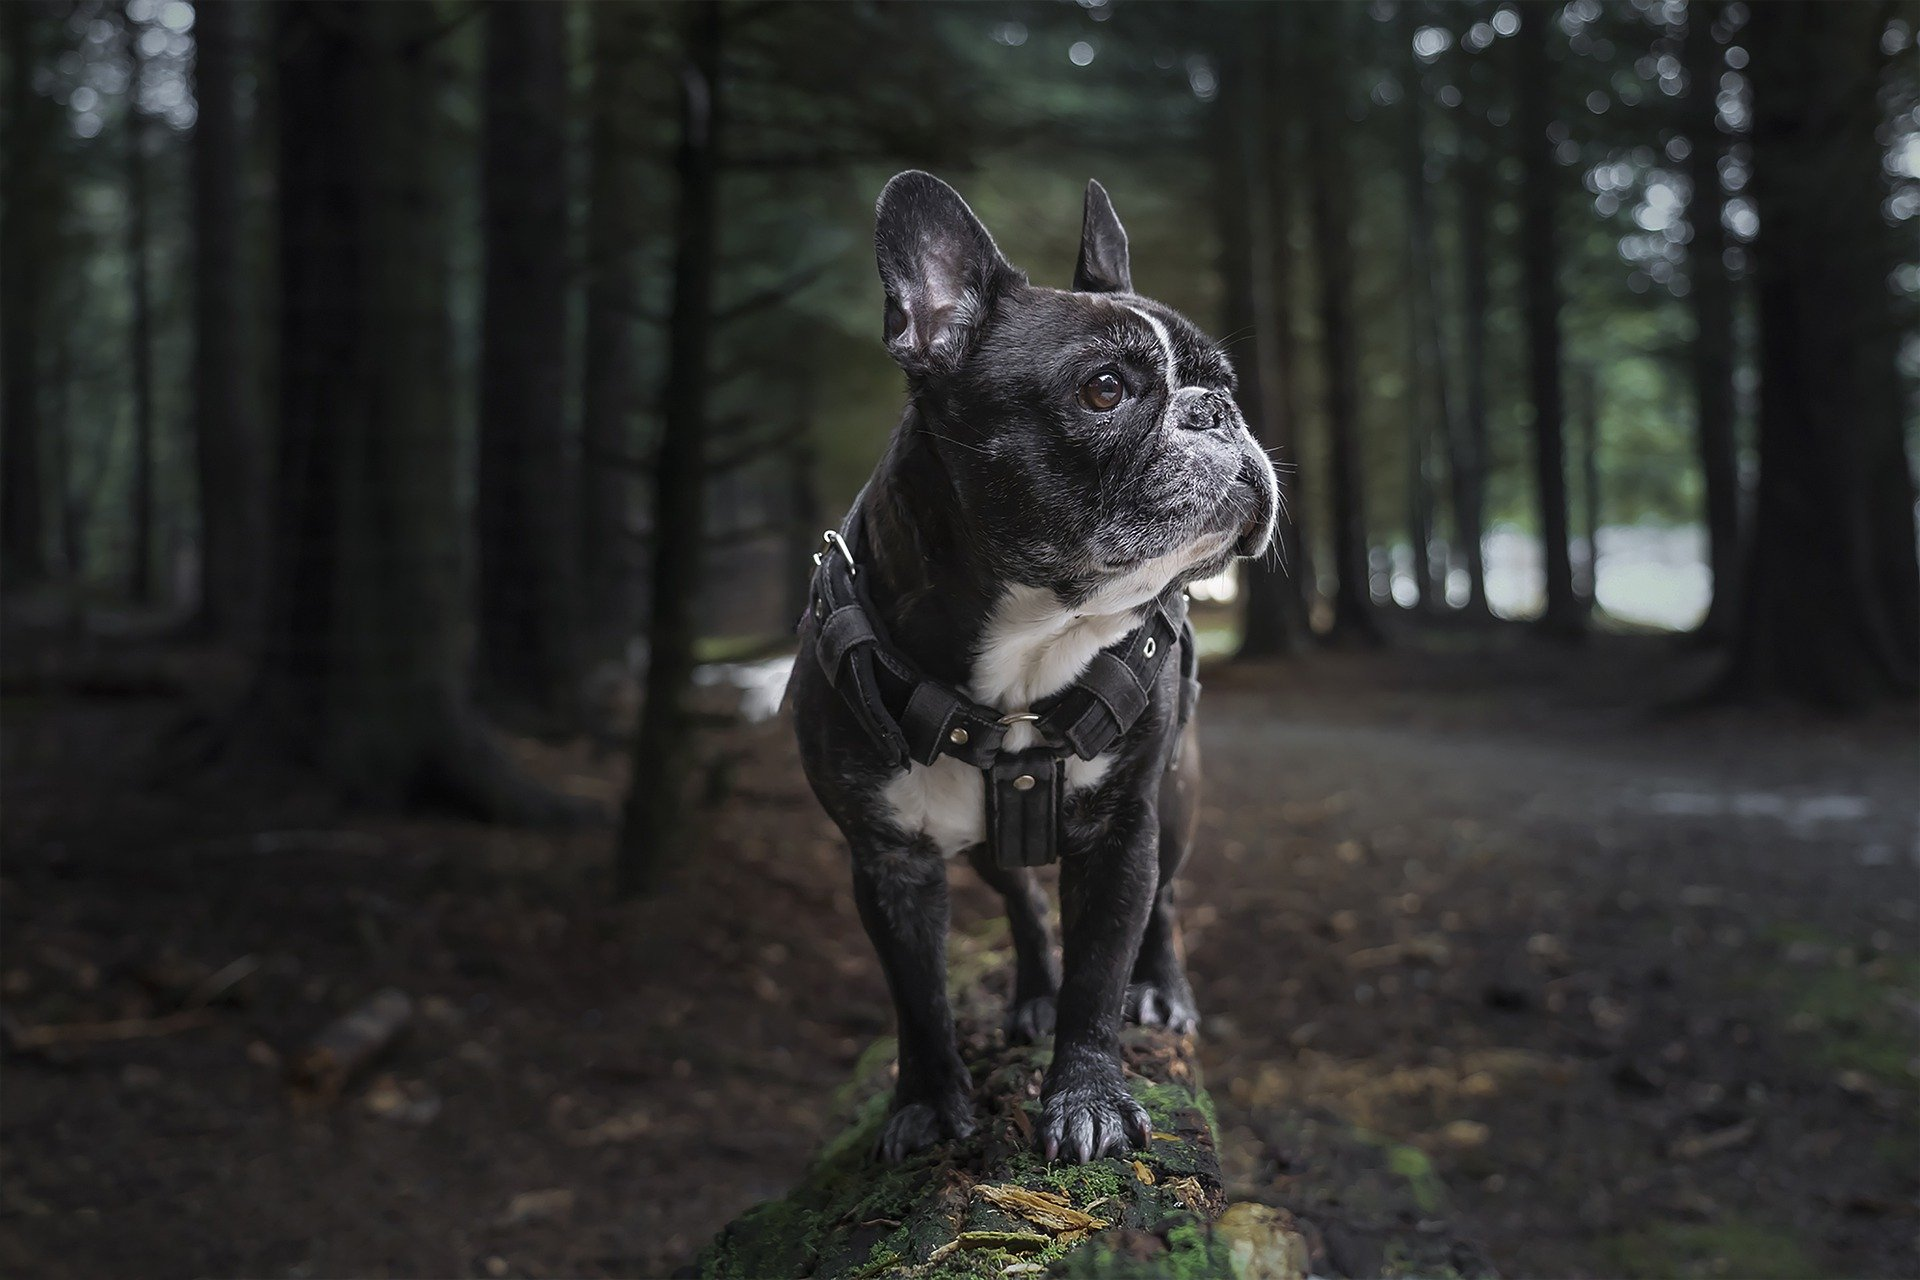
\includegraphics[scale=0.15]{kep}
\caption{A kép leírása}
\end{figure}
\end{frame} 

\begin{frame}{Úsztatott ábrák}
\begin{itemize}
\item Formátum: \\ 
	\tbs begin\{figure\} \\ 
	Az ábra (kép, ...) kódja \\
	\tbs end\{figure\}
\end{itemize}
\vspace{1cm}
\begin{itemize}
\item Összefüggő, nem törhető elemek
\item A \LaTeX{} képes ,,úsztatni'' a megfelelő helyre
\item Címeket is adhatunk nekik a \textbf{\tbs caption\{cím\}} módon.
\end{itemize}
\end{frame}

\begin{frame}[fragile]{A kép, mint úsztatott ábra}
\begin{verbatim}
\begin{figure}
\includegraphics[scale=0.5]{beillesztett_kep}
\caption{A kep leirasa}
\end{figure}
\end{verbatim}
\end{frame}
 
\begin{frame}[fragile]{Úsztatott táblázat}
\begin{verbatim}
\begin{table}
\begin{tabular}{|c||c|}
\hline 
elem1 & elem2 \\ 
\hline \hline
elem3 & elem4 \\ 
\hline 
\end{tabular}
\caption{A táblázat leírása}
\end{table}
\end{verbatim}
\end{frame}

\begin{frame}{Az úsztatás pozicionálása}
\begin{itemize}
\item Lehetőség van a \LaTeX{} számára megmondani, hogy hová szeretnénk úsztatni az ábránkat
\item Ezt az opcionális paraméterekhez kell megadni
	\begin{itemize}
	\item \textbf{h} - az aktuális helyen kerüljön elhelyezésre. Kis ábrák és táblázatok esetén hasznos.
	\item \textbf{t} -  a lap tetején
	\item \textbf{b} - a lap alján
	\item \textbf{p} - egy speciális oldalon, ami csak úsztatott objektumokat tartalmaz
	\item \textbf{!} - mindenképp történjen meg az elhelyezés.
	\end{itemize}
\end{itemize}
\end{frame}

\begin{frame}{Jegyzékek és hivatkozások}
\begin{itemize}
\item A táblázatokat és az ábrákat listázhatjuk is
\item Ezeket a \textbf{\tbs listoffigures} és a \textbf{\tbs listoftables} paranccsal tehetjük meg
\end{itemize}
\vspace{0.5 cm}
\begin{itemize}
\item Ezen kívül hivatkozhatunk  is rájuk
\item Az ábra / táblázat mellé elhelyezett \textbf{\tbs label\{címke\}}-el adjuk meg a hivatkozás tárgyát
\item A szövegben elhelyezett \textbf{\tbs ref\{címke\}}-vel pedig hivatkozunk rá
\item A határozott névelős hivatkozás az \textbf{\tbs aref\{címke\}}
\item A mondat eleji határozott névelős hivatkozás az \textbf{\tbs Aref\{címke\}}
\item Hivatkozni bármire lehet: fejezet, oldal, \dots
\end{itemize}
\end{frame}

\begin{frame}{Lábjegyzet és széljegyzet, url}
\begin{itemize}
\item A szövegbe illeszthetünk lábjegyzeteket is.
\item Ezt a \textbf{\tbs footnote\{Szöveg\}}\footnote{Szöveg} paranccsal tudjuk megtenni.
\item Széljegyzetet a \tbs marginpar\{szöveg\} paranccsal adhatunk meg
\item url címhez szükségünk van a hyperref csomagra
	\begin{itemize}
	 \item \tbs usepackage\{hyperref\}
	\end{itemize}
\item url cím megadásának szintaktikája:
	\begin{itemize}
	\item \tbs href\{url cím\}\{szöveg\}
	\end{itemize}
\item ammennyiben szeretnénk a dokumentumon belül is kattinthatóvá tenni a hivatkozásainkat, ahhoz a hyperref alá az alábbiakat is definiálni kell:
	\begin{itemize}
	\item \tbs hypersetup\{
    colorlinks,
    citecolor=black,
    filecolor=black,
    linkcolor=black,
    urlcolor=black
	\}
	\end{itemize}
\end{itemize}
\end{frame}

\end{document} 
